\documentclass{article}
\usepackage{graphicx} % Required for inserting images
\usepackage{enumitem}
\usepackage{hyperref}


\title{Test 2}
\author{cassadyp }
\date{January 2024}

\begin{document}

\maketitle

\section{Introduction}

\begin{center}
    \textbf{Cassady}
\end{center}

give me information about the damped harmonic oscillator that is a 
car's suspension.

\begin{center}
    \textbf{ChatGPT}
\end{center}

A car's suspension system can be modeled as a damped harmonic oscillator, which is a mechanical system that exhibits both oscillatory (vibratory) and damping (energy dissipation) behavior. The primary purpose of a car's suspension system is to provide a comfortable ride for passengers while ensuring effective handling and stability.
\newline

Here are some key concepts related to the damped harmonic oscillator model for a car's suspension:

\begin{enumerate}
    \item \textbf{Mass (m):} In the context of a car's suspension, the mass refers to the mass of the vehicle body, including the chassis and passengers. The mass is an important parameter as it affects the natural frequency and response of the suspension system.
    \item \textbf{Spring Constant (k):} The spring constant represents the stiffness of the suspension springs. It determines how much force is required to compress or extend the springs. A higher spring constant leads to a stiffer suspension.
    \item \textbf{Damping Coefficient (c):} Damping is crucial in a car's suspension system to control the oscillations of the springs. The damping coefficient represents the amount of damping present in the system. Damping dissipates energy and reduces the amplitude of oscillations, contributing to a smoother ride.
    \item \textbf{Natural Frequency ($\omega_o$):} The natural frequency of the system is the frequency at which the system would oscillate if there were no damping or external forces. It is determined by the mass and the spring constant and is a crucial factor in determining the ride quality.
    \item \textbf{Equation of Motion:} The equation of motion for a damped harmonic oscillator is typically represented as: \newline

    $m\frac{\texttt{d}^2x}{\texttt{d}t^2}+c\frac{\texttt{d}x}{\texttt{d}t}+kx=F(t)$\\

    where:
    \begin{itemize}[label=$\circ$]
            \item $m$ is the mass,
            \item $c$ is the damping coefficient,
            \item $k$ is the spring constant,
            \item $x$ is the displacement of the suspension,
            \item $t$ is time,
            \item $F(t)$ is the external force applied to the system.    
    \end{itemize}
    \item \textbf{Response to Disturbances:} The damped harmonic oscillator model helps in understanding how the suspension system responds to various road disturbances, such as bumps, potholes, or sudden acceleration/deceleration.
    \item \textbf{Tuning for Performance:} Car manufacturers tune the suspension system by adjusting parameters such as spring rates, damping coefficients, and geometry to achieve a balance between comfort and performance. Different types of vehicles (e.g., sports cars, sedans, SUVs) may have different suspension characteristics based on their intended use.\\

    Understanding the damped harmonic oscillator model is essential for designing suspension systems that provide a comfortable and controlled ride while maintaining vehicle stability and handling.
\end{enumerate}

\begin{center}
    \textbf{Cassady}
\end{center}

can you give me a solution for $m$=300kg, $k$=16000N/m, and $c$=1900Ns/m? 

\begin{center}
    \textbf{ChatGPT}
\end{center}

Certainly! To find the solution for the damped harmonic oscillator with the given values of mass ($m$=300kg), spring constant ($k$=16000N/m), and damping coefficient ($c$=1900Ns/m), we can use the differential equation for a damped harmonic oscillator:\\
\\
$m\frac{\texttt{d}^2x}{\texttt{d}t^2}+c\frac{\texttt{d}x}{\texttt{d}t}+kx=0$\\
\\
with the given values, the equation becomes:\\
\\
$300\frac{\texttt{d}^2x}{\texttt{d}t^2}+1900\frac{\texttt{d}x}{\texttt{d}t}+16000x=0$\\
\\
This is a second-order linear homogeneous ordinary differential equation. The general solution to this type of equation can be expressed as a combination of exponential functions:\\
\\
$x(t)=e^{ -\frac{c}{2m}t } \left( Acos \left( \sqrt{ \frac{k}{m}-\left(\frac{c}{2m}\right)^2 }t \right) + Bsin \left( \sqrt{ \frac{k}{m} - \left( \frac{c}{2m} \right)^2}t \right) \right)$\\
\\
where $A$ and $B$ are constants that depend on the initial conditions of the system.\\
\\
If you have specific initial conditions (such as initial displacement $x_o$ and initial velocity $v_o$), you can use them to determine the values of $A$ and $B$ and obtain a particular solution for the given scenario.\\
\\
Keep in mind that the damping in the system ($c$) affects the behavior of the solution. For stronger damping, the oscillations are damped more quickly, leading to a quicker return to the equilibrium position but with reduced amplitude.

\begin{center}
    \textbf{Cassady}
\end{center}

what if the initial displacement is 1 meter and the initial velocity is 0?

\begin{center}
    \textbf{ChatGPT}
\end{center}

If the initial displacement ($x_o$) is 1 meter and the initial velocity ($v_o$) is 0, you can use the general solution for a damped harmonic oscillator and apply the initial conditions to determine the constants A and B \footref{fig:1}. The general solution is given by:\\
\\
$x(t)=e^{ -\frac{c}{2m}t } \left( Acos \left( \sqrt{ \frac{k}{m}-\left(\frac{c}{2m}\right)^2 }t \right) + Bsin \left( \sqrt{ \frac{k}{m} - \left( \frac{c}{2m} \right)^2}t \right) \right)$\\
\\
Given the initial conditions:\\
$x(0)=x_o$ and $v(0)=v_o$\\
\\
Substituting these into the solution:\\
\\
$x(0)=Acos(0)+Bsin(0)=A$\\
\\
$v(0)=\left(-\frac{c}{2m} \right) Asin(0) + \sqrt{ \frac{k}{m}- \left( \frac{c}{2m} \right)^2} Bcos(0) = \sqrt{ \frac{k}{m} }B$\\
\\
Since $x_o=A$ and $v_o=\sqrt{ \frac{k}{m} }B$,\\
\\
you can find A and B as follows:\\
\\
$A=x_0=1$meter $B=\frac{v_o}{\sqrt{\frac{k}{m}}}=\frac{0}{\sqrt{16000*300}}=0$\\
\\
Therefore, in this case, the constants A and B simplify, and the solution for the displacement $(x(t))$ becomes:\\
\\
$x(t)=e^{-\frac{c}{2m}t} cos \left( \sqrt{ \frac{k}{m} - \left(\frac{c}{2m}\right)^2 } \right)$\\
\\
You can plug in the values for m, k, and c to obtain the specific solution for your scenario.

\begin{figure}[h]
    \centering
    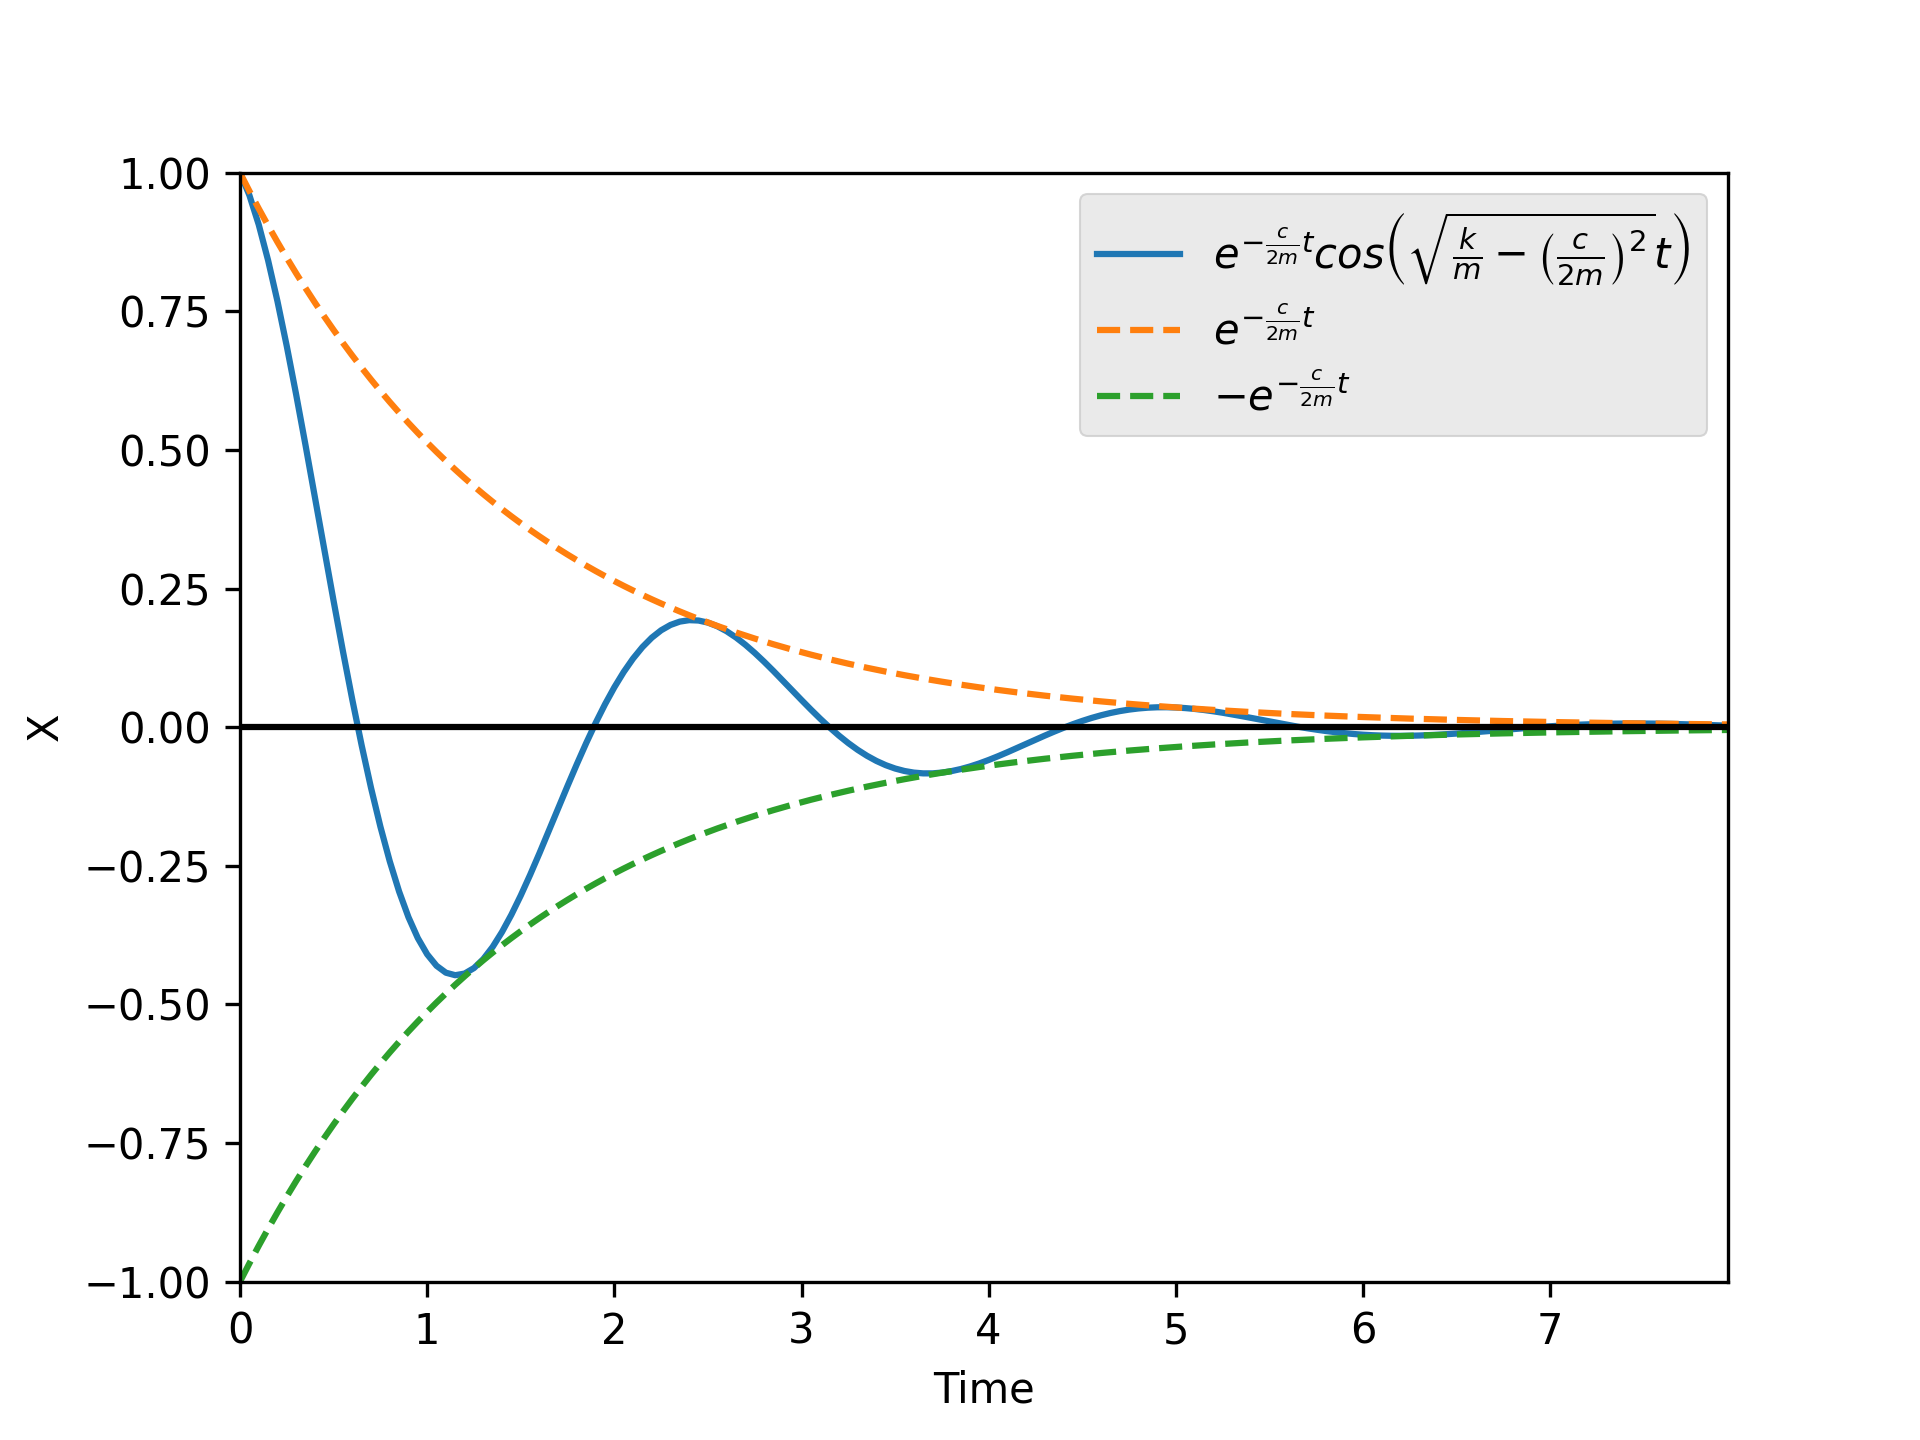
\includegraphics{Figure1.png}
    \caption{$m=300$kg, $c=400$Ns/m, and $k=2000$N/m}
    \label{fig:1}
\end{figure}

\end{document}
